\chapter{Sammeln der Daten}
\label{Kapitel5}

Das folgende Kapitel bietet die Einleitung in die Durchführung und beschäftigt sich mit der Datenaufnahme. Hierfür wird zuerst für das Mikrofon eine spezielle eigens angefertigten Halterung konstruiert, dann der Aufbau des Roboters mitsamt des Aufnahme Equipments erläutert und zum Schluss eine Abschnitt über die Durchführung der Aufnahme. Abschließend folgt eine Bewertung über die Probleme und Erfolge bei der Datenaufnahme, bevor dann im nächsten Kapitel die tatsächliche Analyse stattfindet

\section{Konstruktion der Mikrofonhalterung}

Der Entwurf der Mikrofonhalterung begann mit einem simplen Klemmmechanismus als Prototyp. Dieser Mechanismus wurde jedoch aufgrund mangelnder Stabilität schnell verworfen. Anstelle einer einfachen Klemme wurden zwei Halbbögen verwendet, die etwas weniger als die Hälfte des Umfangs des Quickchangers umfassten, an welchem die Halterung dann befestigt wurde. Dadurch konnte die Halterung mittels Schrauben mit Druck zusammengespannt werden, was zu einer deutlich verbesserten Stabilität führte. Zudem erlaubt es der Mikrofonhalterung am Roboterarm um 360° um diesen gedreht zu werden, was weitere Bewegungsfreiheit gewährleistete.

Der nächste Schritt war die Entwicklung des Mikrofonarms. Dieser sollte maximale Freiheit bei der Positionierung des Mikrofons bieten. Daher entschied man sich für zwei Teilarme, die jeweils mit einer Schraube verbunden wurden. Dies ermöglichte eine flexible Positionierung des Mikrofons, vor allem in der Nähe des Schleifers.

Der letzte Teilarm diente als Befestigungspunkt für die offizielle Mikrofon klammer. Das Mikrofon wurde an dieser Klammer angebracht und konnte sich nur um seine eigene Achse drehen. Dabei stand das Mikrofon stets senkrecht zum Roboterarm und zur Schleifmaschine. Eine Anpassung dieses Winkels war nicht nötig, da die Position durch die zwei Teilarme flexibel und präzise eingestellt werden konnte.

\begin{figure}[H]
    \centering
    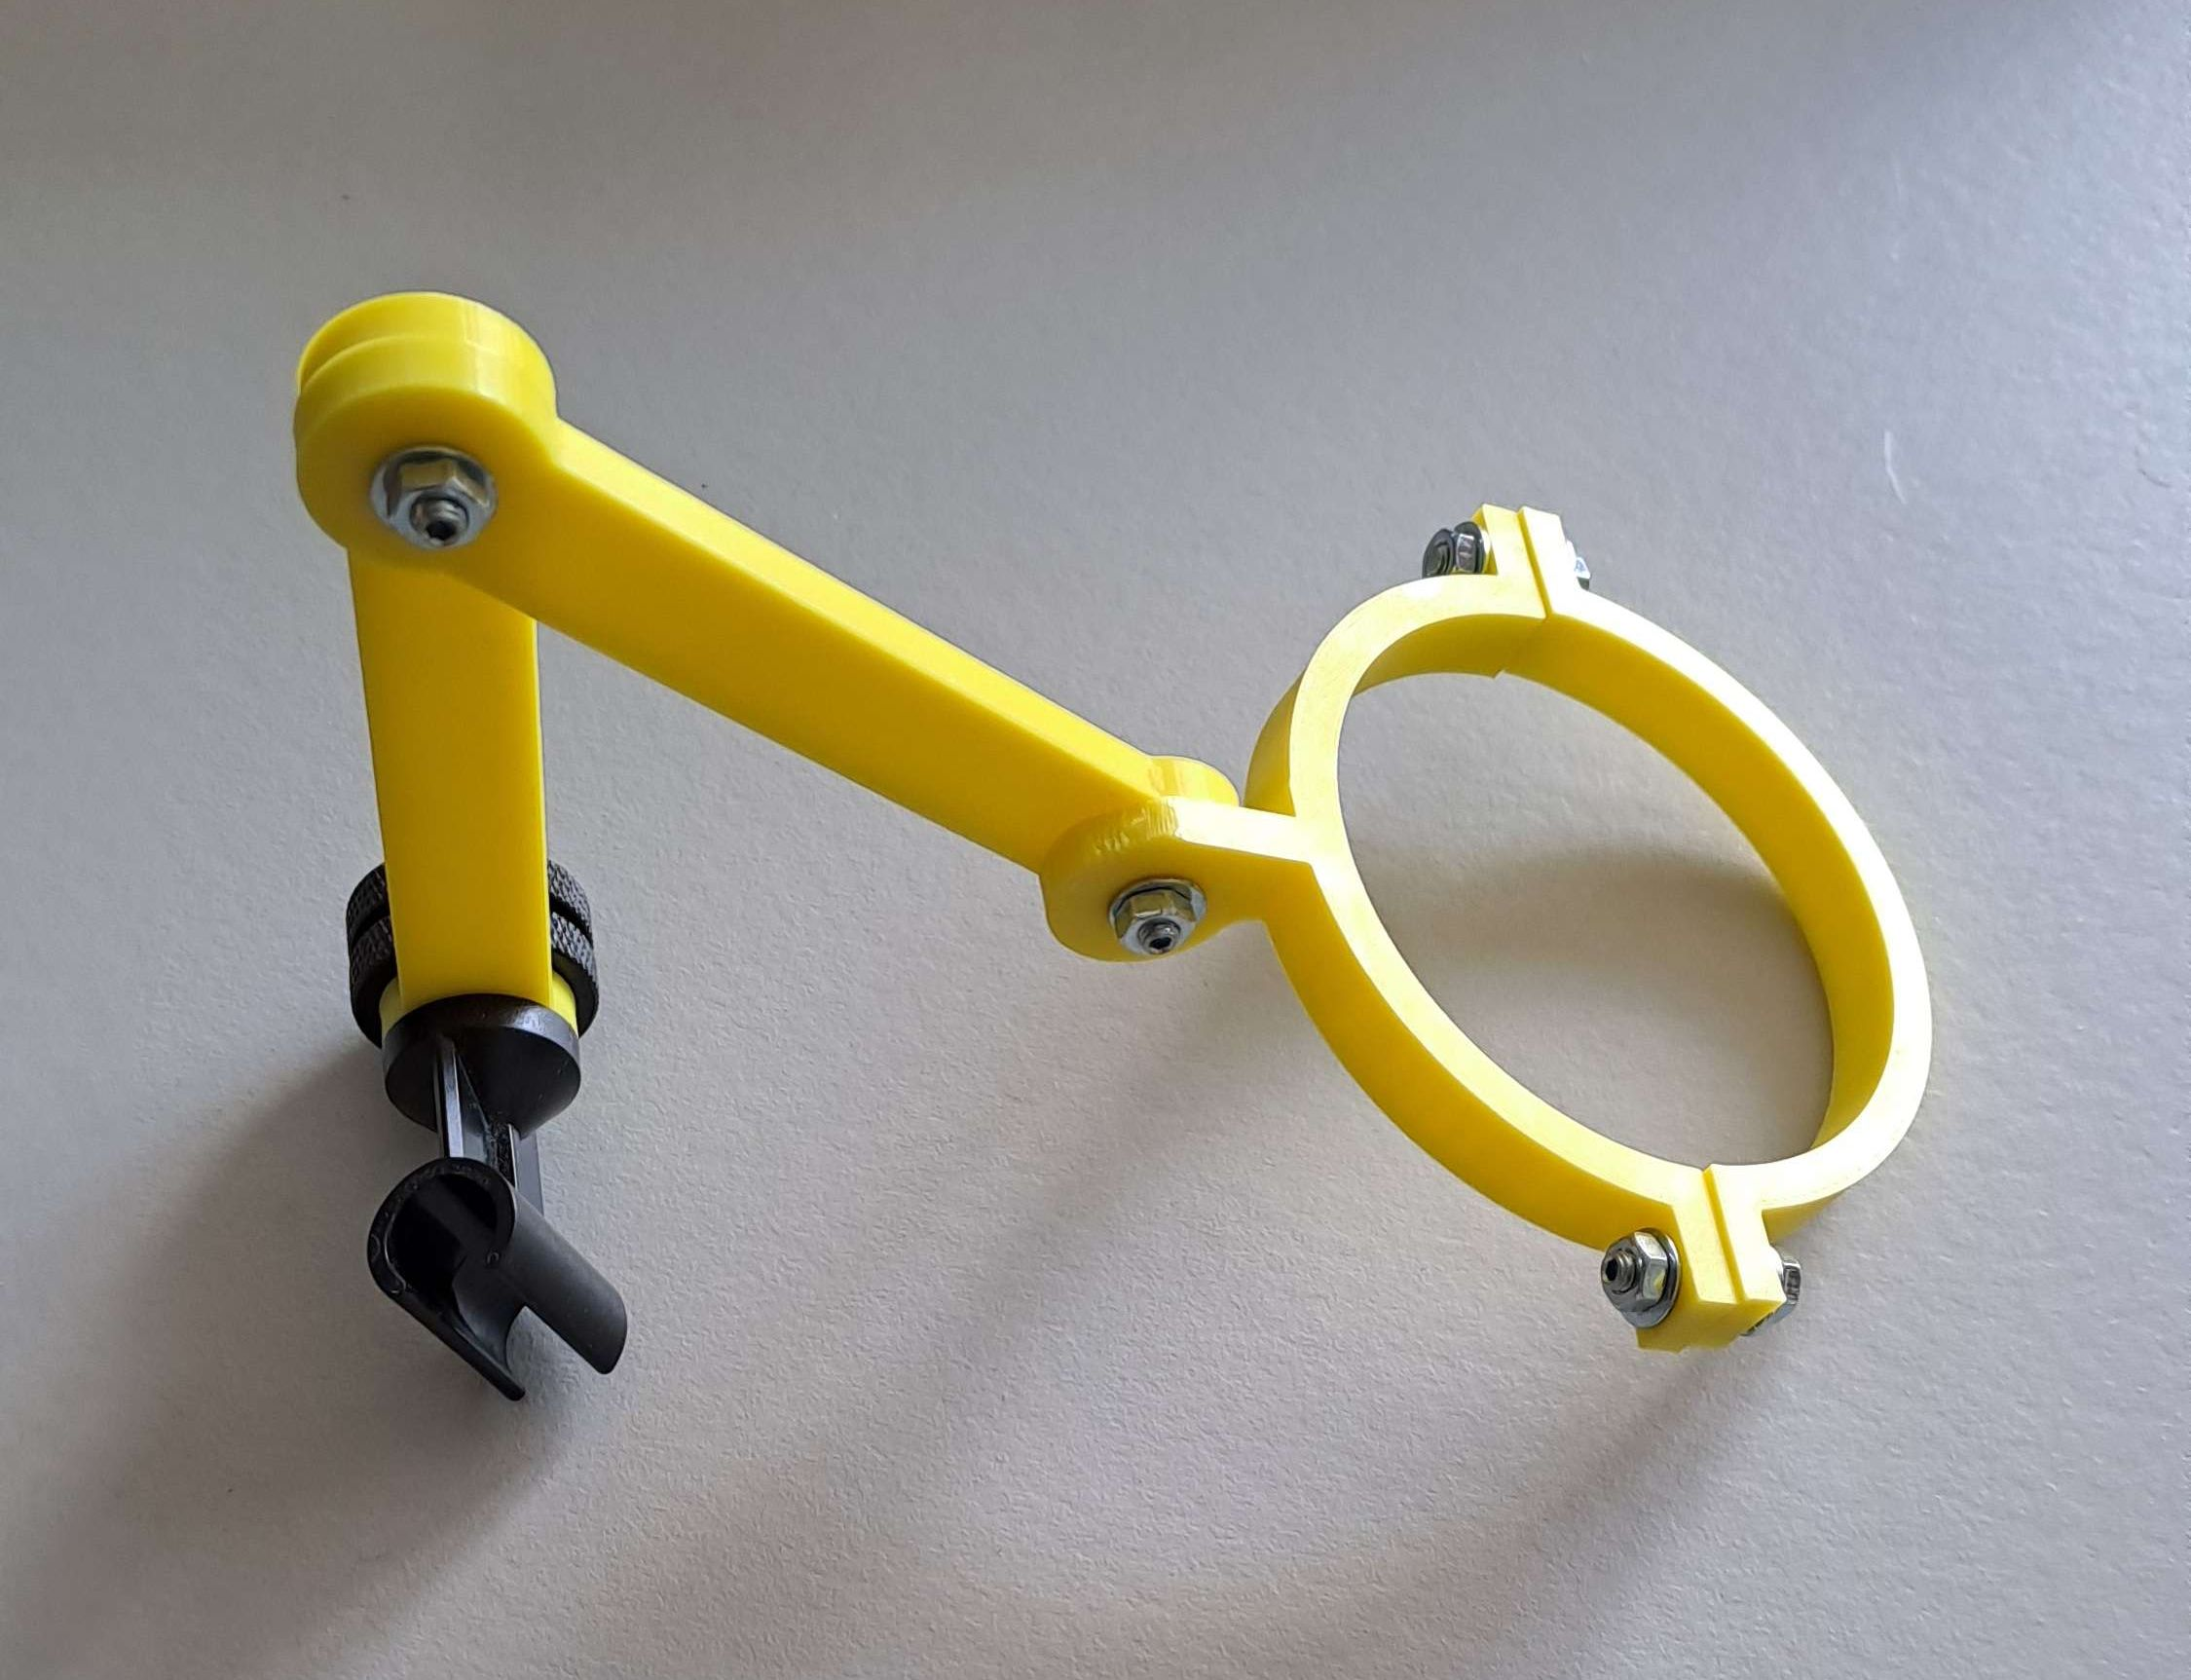
\includegraphics[width=0.5\linewidth]{images/Mikrofonhalterung.jpg}
    \caption{Fertige Mikrofonhalterung}
    \label{fig:Mikrofonhalterung}
\end{figure}

\section{Aufbau}

\begin{figure}[H]
    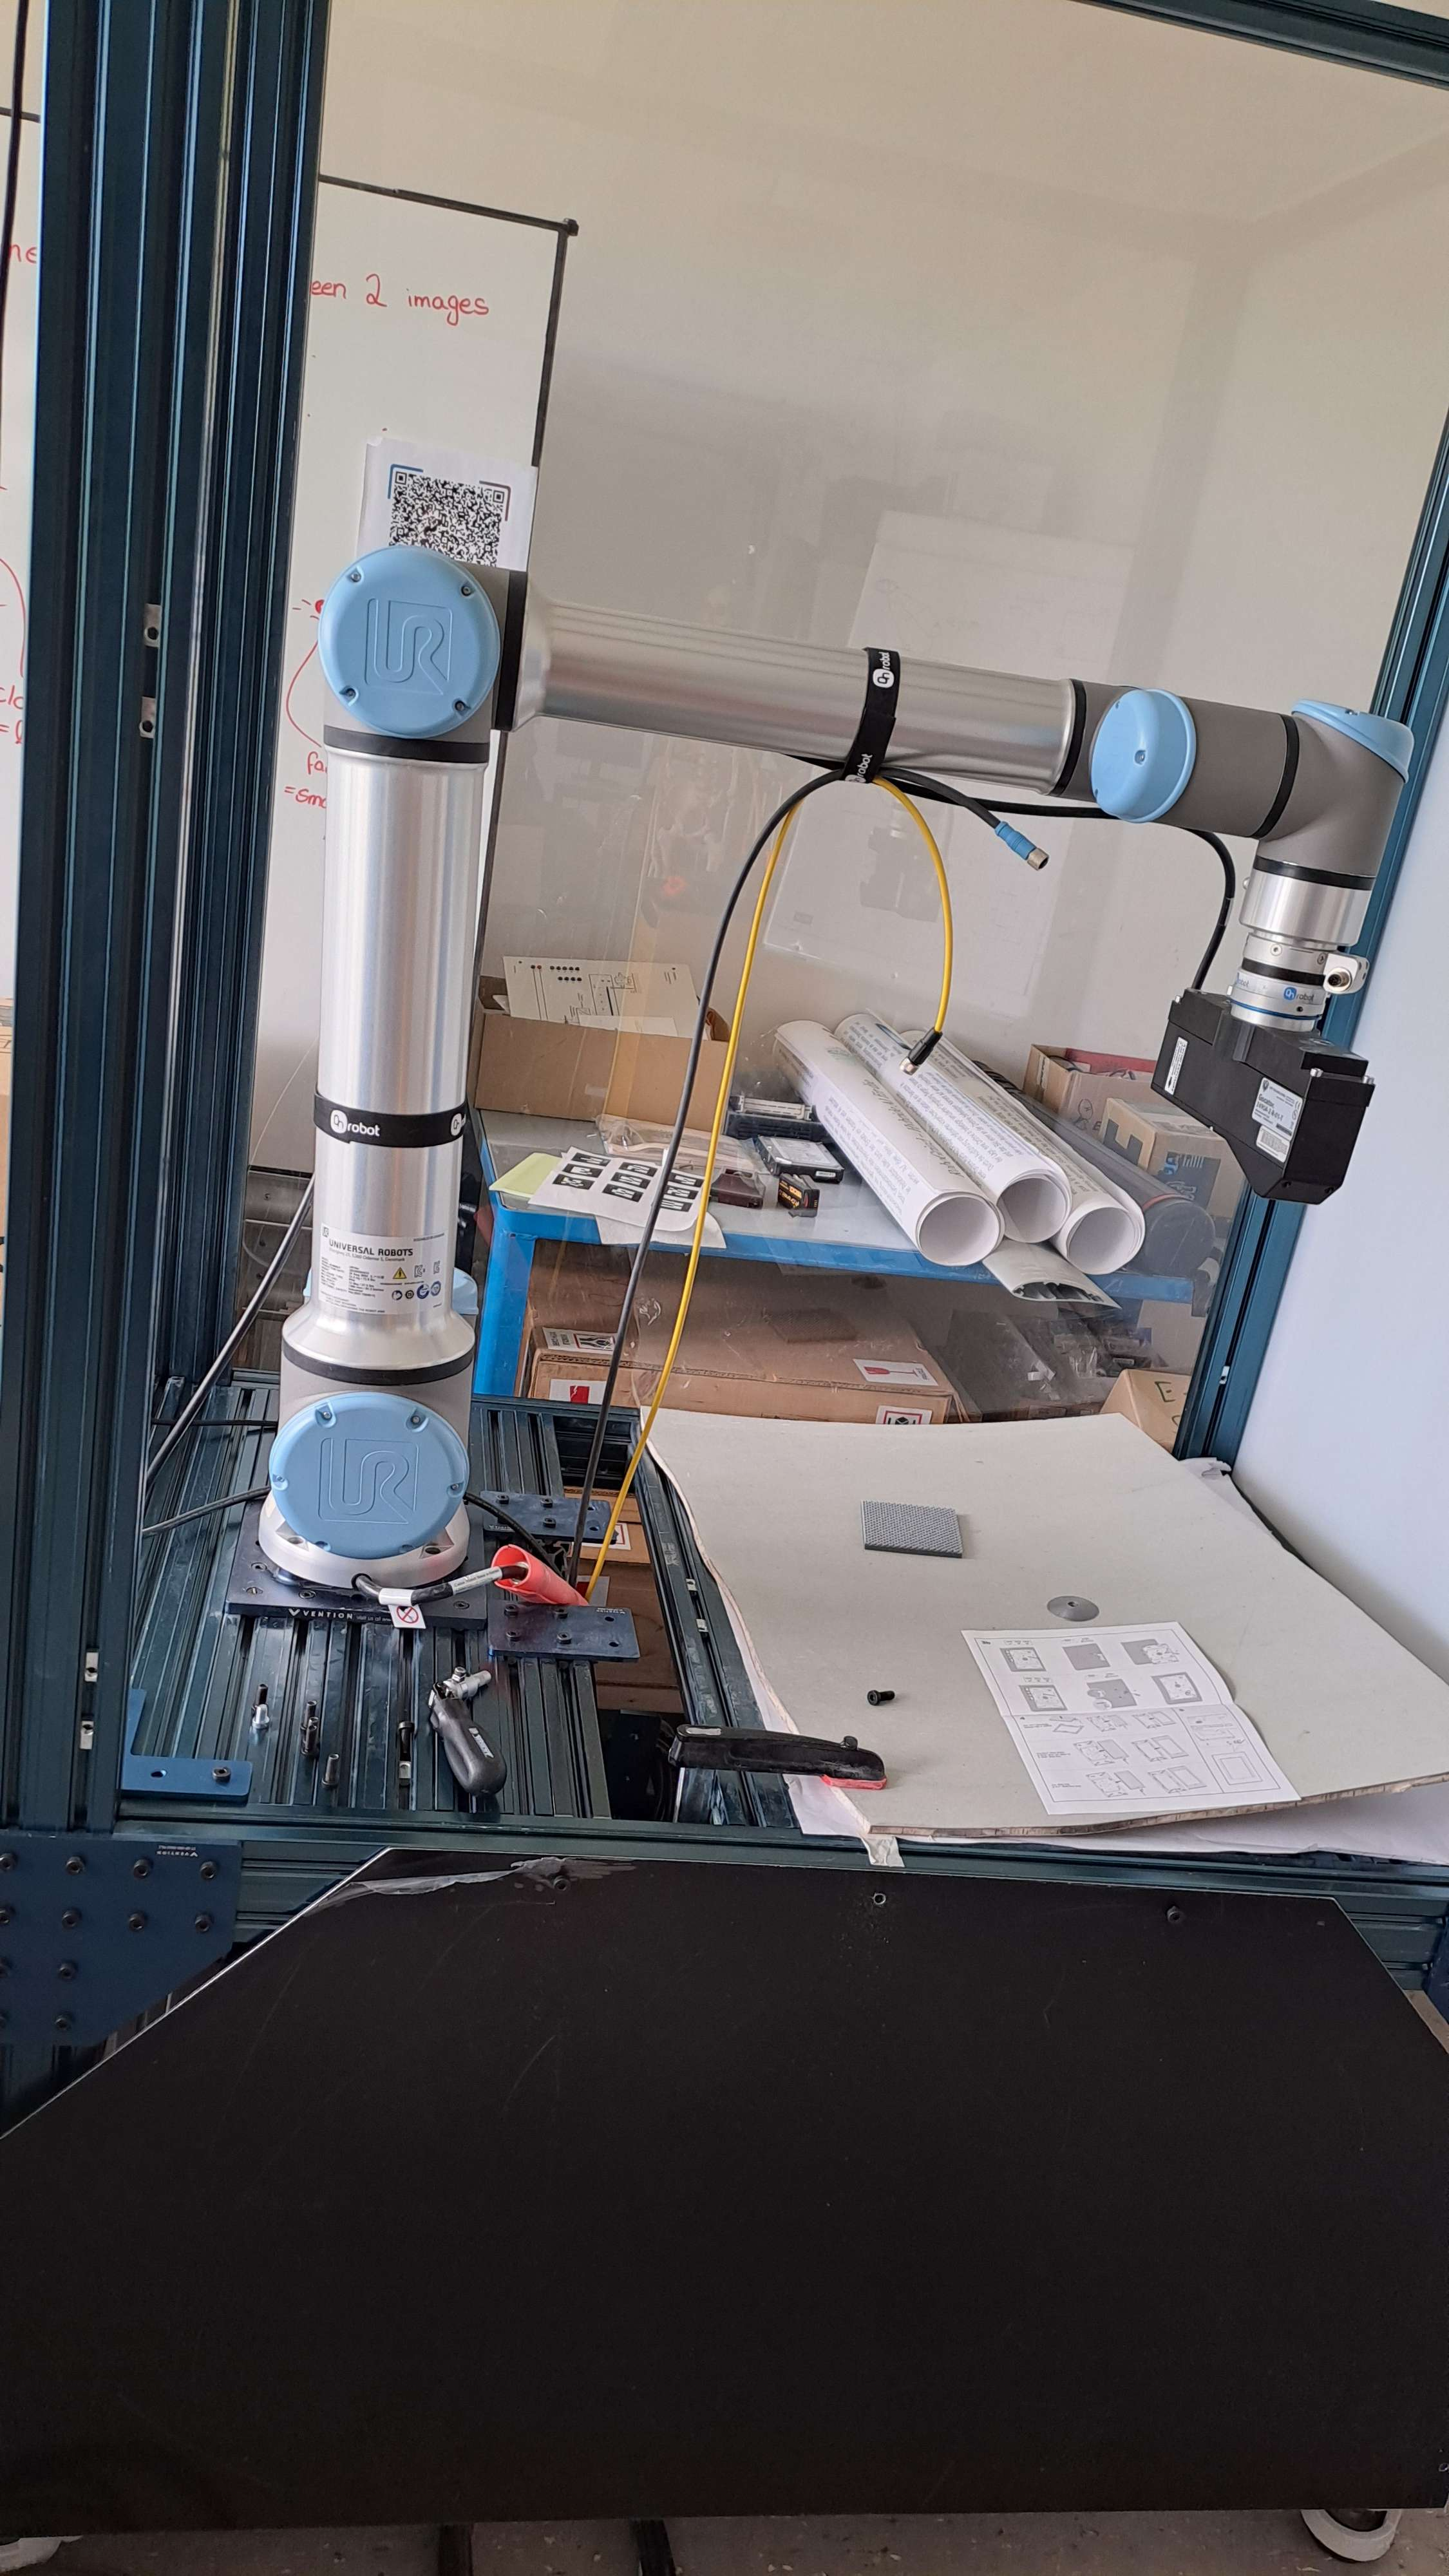
\includegraphics[width=0.5\linewidth]{images/Roboter.jpg}
    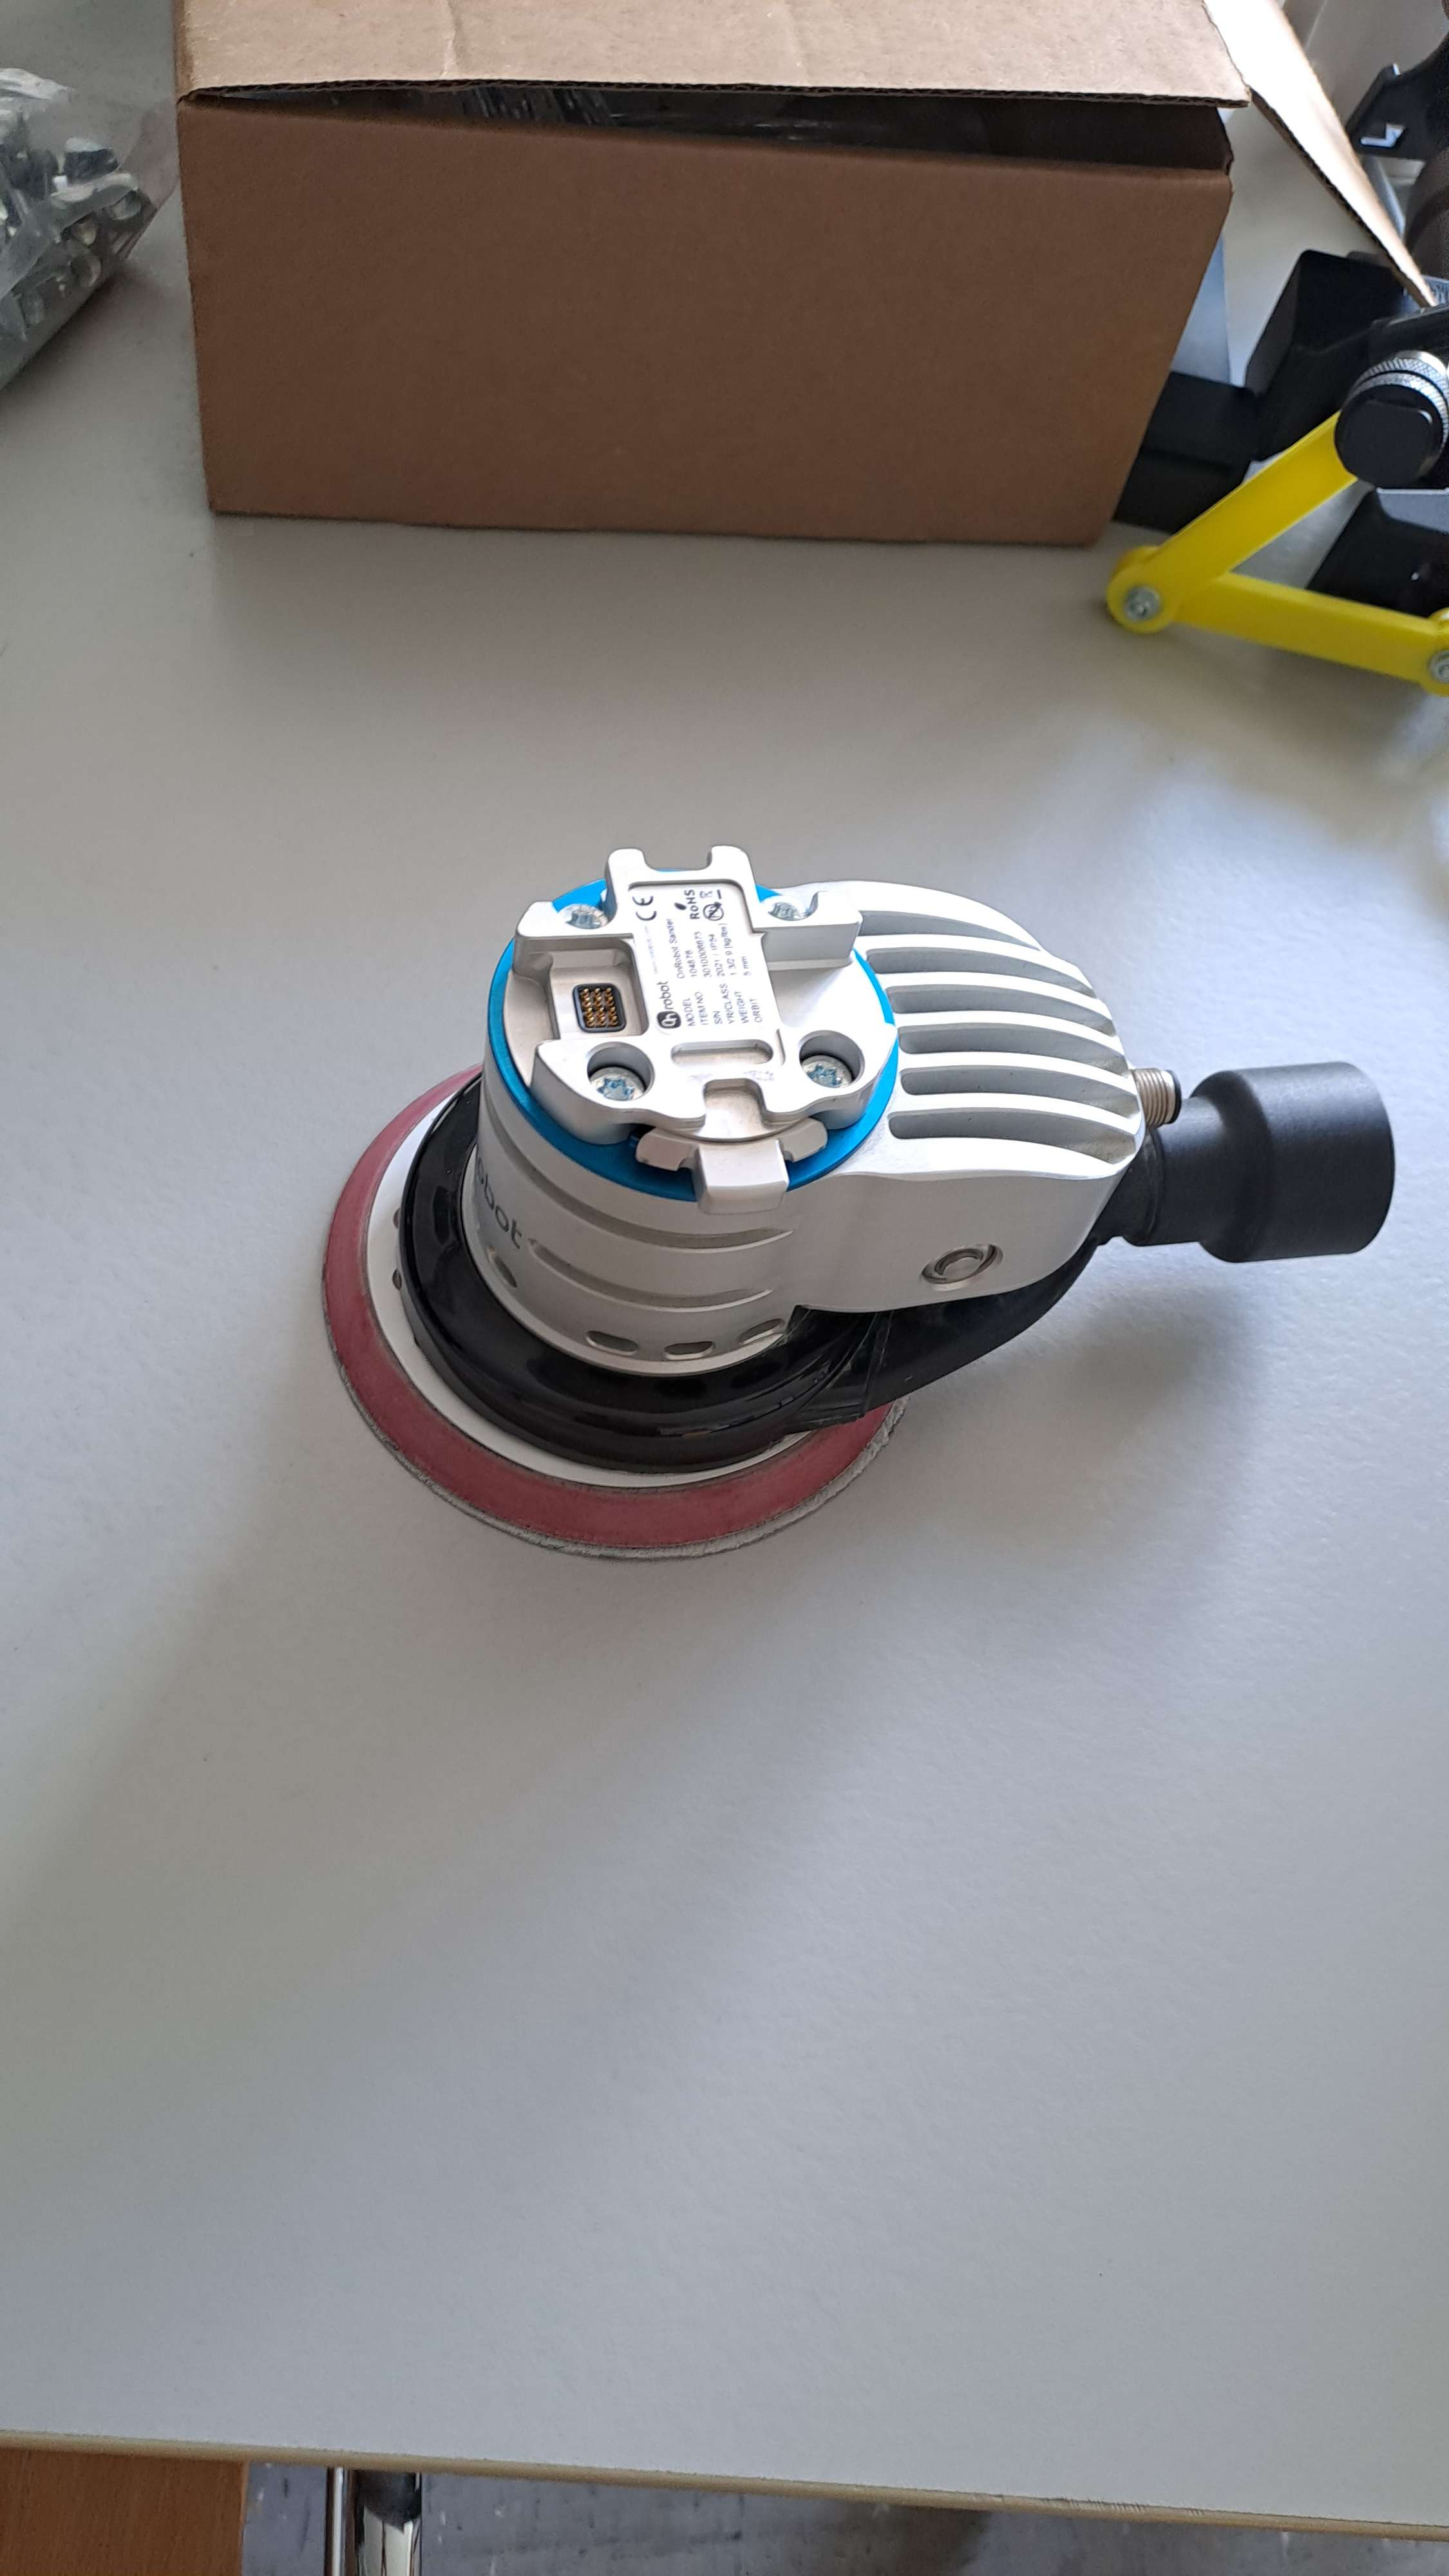
\includegraphics[width=0.5\linewidth]{images/Schleifer.jpg}
    \caption{Roboter und Schleifer}
    \label{fig:Roboter und Schleifer}
\end{figure}

Der Aufbau beinhaltet einen Industrieroboter vom Typ UR10e von Universal Robots. Diese Steuerung des UR10e erfolgt über eine spezielle Software, die es ermöglicht, den Roboter über ein graphisches Benutzerinterface zu programmieren. Diese Software bietet Flexibilität bei der Definition von Bewegungsbahnen, die entweder vorprogrammiert oder während des Betriebs manuell angepasst werden können. Um eine Konsistenz zu gewährleisten wurden mehrere automatische Bahnen programmatisch festgelegt, die den Roboter in definierten Mustern über die Werkstückoberfläche führen. Nach der initialen Konfiguration wurden mehrere Testläufe durchgeführt, um die korrekte Funktion der programmierten Bewegungsbahnen zu überprüfen. Der Roboter operiert innerhalb eines abgeschlossenen Glaskastens, der effektiv den Schleifstaub eingrenzt und den Lärmpegel reduziert, wodurch eine sichere und kontrollierte Arbeitsumgebung gewährleistet wird.

Für den Schleifprozess ist der Roboterarm mit einem OnRobot-104876 Electric Random Orbital Sander ausgestattet, der mittels eines OnRobot-109498 HEX-E Quickchangers befestigt ist. Das verwendete Schleifpapier hat eine Körnung von 120 und war wie neu, ideal für das gleichmäßige Schleifen des Werkstücks, einem Teil eines Windradblattes aus einem Gemisch aus Glasfaser und Holz.

Zur akustischen Überwachung des Schleifvorgangs wurde ein Mikrofon vom Typ M2010 der Marke NTi Audio in einem Abstand von 10-15 mm zum Schleifkopf angebracht. Dieses ist auf dem bereits beschriebenen und in der Abbildung \ref{fig:Mikrofonhalterung} gezeigten 3D gedruckten Mikrofonarm montiert und mit einem Mikrofon-Windschutz (Puschel) ausgestattet, der Störgeräusche wie Luftbewegungen bereits von alleine reduziert.

Die aufgenommenen Audiosignale werden über ein Audiomixer an einen Laptop weitergeleitet, wo sie mit der Software Audacity aufgezeichnet werden. Die Aufzeichnung erfolgt mit einer Abtastrate von 44,1 kHz und einer Bit-Tiefe von 16 Bit, was eine hohe Qualität der Datenerfassung sicherstellt. Diese waren jedoch zu detailliert weswegen diese im Verlauf der Bearbeitung auf 8 kHz Abtastrate heruntergesampelt wurden.

\section{Durchführung}

Bevor der Roboter den Schleifvorgang starten kann, wird der Schleifkopf mit dem passenden Schleifpapier (Körnung 120) bestückt und sicher an der OnRobot-109498 HEX-E Quickchanger-Aufhängung montiert. Anschließend wird das geplante Schleifprogramm auf das Steuerungstablet des UR10e-Roboters geladen und konfiguriert. Hierbei wird insbesondere auf die korrekten Einstellungen für Schleifbahnen, Anpressdruck und Schleifgeschwindigkeit geachtet. Parallel dazu wird die Aufnahmesoftware Audacity auf dem Laptop gestartet. Das Mikrofon wird über Audiomixer an den Laptop angeschlossen. Nachdem die Einstellungen für die Aufnahmesoftware überprüft wurden, wird die Aufnahme gestartet. Dabei wird darauf geachtet, dass die Aufnahmepegel korrekt eingestellt sind, um Übersteuerung zu vermeiden. Sobald die Aufnahme läuft, wird das vorbereitete Schleifprogramm auf dem Roboter gestartet. Der UR10e führt den Schleifprozess entlang der vorgegebenen Bahnen durch und bearbeitet das gebogene Werkstück gleichmäßig mit konstanter Schleifkraft. Die Audiospur in Audacity sieht dann wie folgt aus:

\begin{figure}[H]
    \centering
    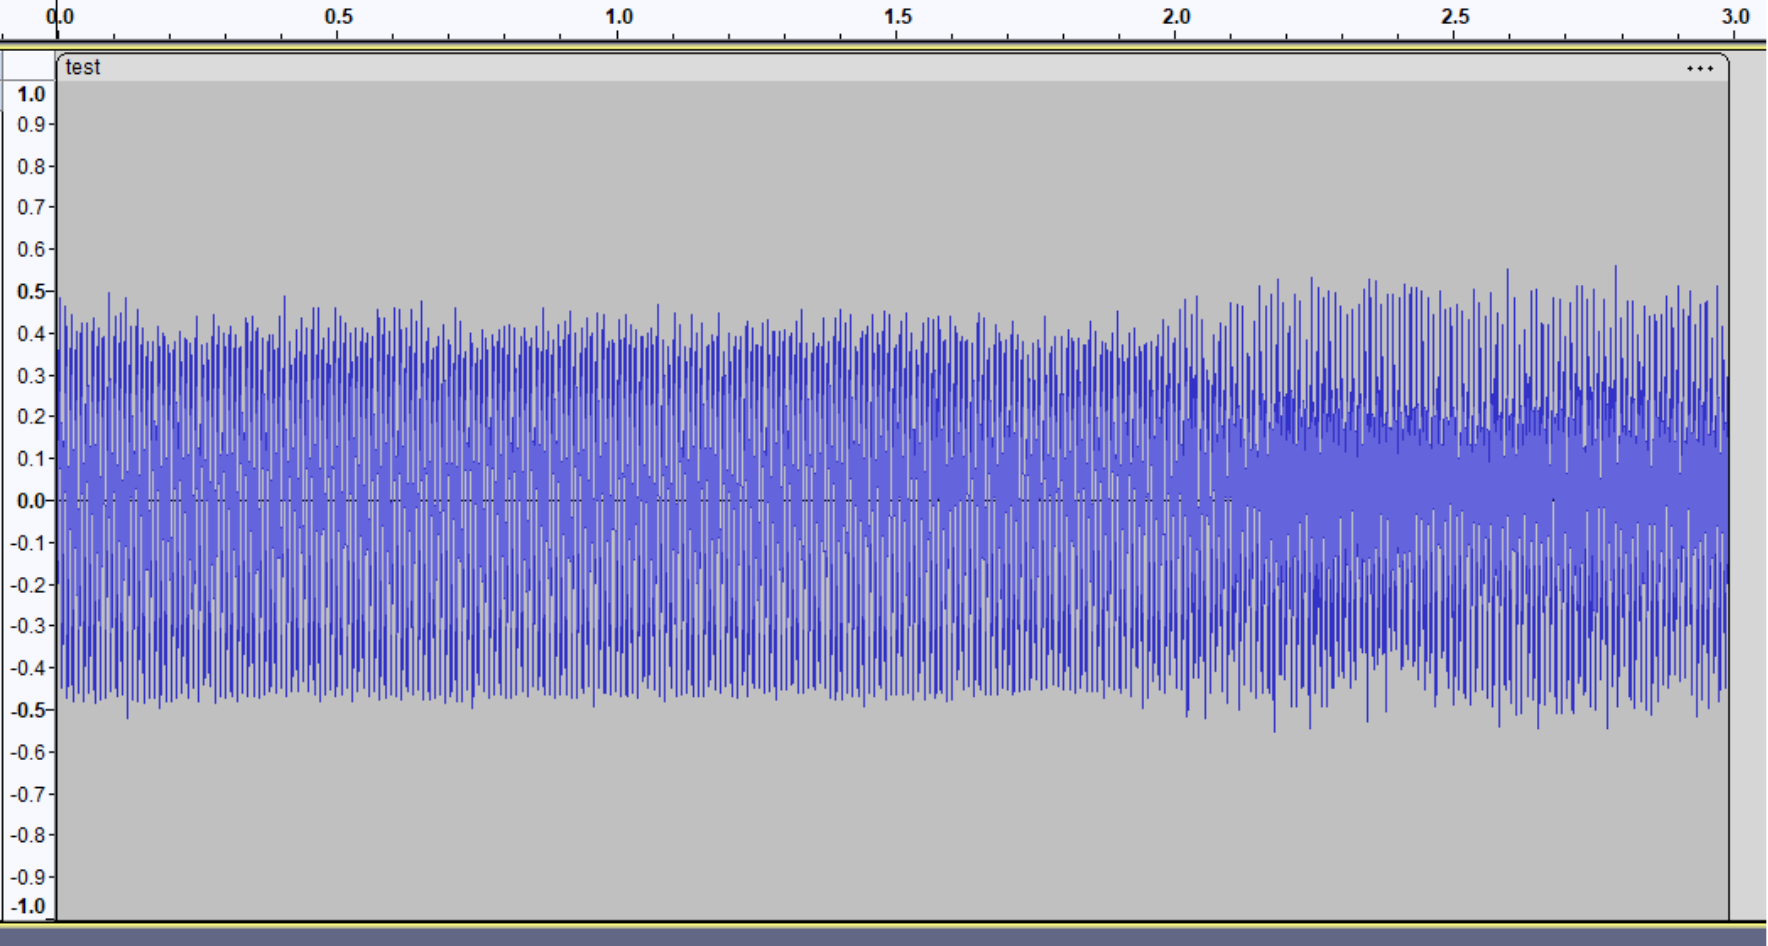
\includegraphics[width=0.7\linewidth]{images/audacity.png}
    \caption{Visualisierung eines Audiosignals in Audacity}
    \label{fig:enter-label}
\end{figure}

Die Aufnahme dauert etwa eine Minute und erfasst den gesamten Schleifvorgang. Sollte während des Schleifens etwas schiefgehen, wie ein zu hoher Anpressdruck, der den Schleifprozess beeinträchtigt, wird die Aufnahme vorzeitig abgebrochen. In diesem Fall wird das Problem identifiziert und behoben, bevor ein neuer Aufnahmeversuch gestartet wird. Nach Abschluss der Aufnahme wird die Audiodatei entsprechend der Einstellungen des Schleifprozesses betitelt und in einer Excel-Tabelle erfasst. Diese Tabelle enthält Informationen zu den verwendeten Schleifprogrammen, Umdrehungszahl, besonderen Ereignissen und weiteren relevanten Parametern, um einen einfachen Überblick über die Aufnahmen zu behalten.     

\section{Auswertung}

Das automatische Schleifen durch vorprogrammierte Bahnen hat nicht immer konsistent funktioniert, da dort mit einer konstanter Kraft nach unten gedrückt wird, was bei einem schrägen Werkstück dazu führt, dass der Schleifer langsam kippt. Bei dem manuellen Schleifen war es allerdings nicht möglich konstistent zu schleifen, da dort die Steuerung deutlich schwieriger ist, was oftmals dazu geführt hat, dass der Anpressdruck bei Beginn des Schleifvorgangs zu hoch war. Weiterhin ist durch die nun nicht mehr automatische Anpressdruckkontrolle dieser über die Breite des Schleifstücks nicht konstant. 

Neben dem Schleifen war auch das Mikrofon anfangs nicht fest genug angebracht, sodass dieses sich durch das Vibrieren des Roboters beim Schleifen langsam abgesenkt hat und somit die Distanz zum Schleifer leicht verändert wurde. Nach erneutem Festziehen der Schrauben war dieses Problem aber gelöst.


%%%%%%%%%%%%%%%%%%%%%%%%%%%%%%%%%%%%%%%%%%%%%%%%%%%%%%%%%%%%%%%%%%%%%%%%%%%%%%%
\endinput
%%%%%%%%%%%%%%%%%%%%%%%%%%%%%%%%%%%%%%%%%%%%%%%%%%%%%%%%%%%%%%%%%%%%%%%%%%%%%%%
